% =====================================================================
%  Springer LNCS submission — conference-ready version of Paper A
%  Compile on Overleaf: New Project -> Upload Project -> upload this
%  whole folder (main.tex + figures/).  Menu -> Compiler -> pdfLaTeX.
%
%  This uses the official Springer LNCS class (llncs).  Overleaf has it
%  built in; no need to add llncs.cls yourself.  The same layout is used
%  for LNNS (Lecture Notes in Networks and Systems), so this file works
%  for both ICAIC (Springer) and ICDMIS (Springer LNNS).
% =====================================================================
\documentclass[runningheads]{llncs}

\usepackage{graphicx}
\usepackage{amsmath}
\usepackage{booktabs}
\usepackage[T1]{fontenc}
\usepackage{textcomp}      % for \$, degree, etc.

% Running head (short title) shown at top of pages
\begin{document}

\title{NISQ Noise Shifts the Quantum Amplitude\\ Estimation Break-Even for Option Pricing}

% If the venue wants a short running title, this is it:
\titlerunning{NISQ Noise Shifts the QAE Break-Even for Option Pricing}

\author{Prithvi Raghu}
\authorrunning{P. Raghu}

\institute{Vellore Institute of Technology, Vellore, India\\
\email{prithviraghu080706@gmail.com}}

\maketitle

\begin{abstract}
Quantum amplitude estimation (QAE) is widely cited as offering a quadratic
speedup over classical Monte Carlo for derivative pricing, with the canonical
break-even occurring when the QAE oracle-query budget $M$ falls below the
classical sample budget $N$. Nearly all such analyses assume noiseless quantum
hardware. We quantify how realistic depolarizing noise degrades QAE-based
European call pricing across a 50-point parameter sweep at five noise levels
($p \in \{0, 10^{-4}, 10^{-3}, 5\times10^{-3}, 10^{-2}\}$) using iterative QAE
(IQAE) with three uncertainty qubits on a depolarizing-noise simulator,
validated against a single-qubit state-preparation run on IBM hardware
(\texttt{ibm\_marrakesh}). We report three findings. First, at the current IBM
hardware noise level ($p \approx 10^{-3}$) the mean absolute price error is
\$0.657 --- roughly $66\times$ the $\varepsilon = 0.01$ precision target that
defines the theoretical break-even. Second, and more strikingly, even at
$p = 0$ the mean error is \$0.203, already ${\approx}20\times$ above target:
the three-qubit discretization imposes an irreducible approximation error
before any noise is introduced, so the asymptotic advantage is unattainable on
near-term devices regardless of noise. Third, the IQAE oracle-query depth is
noise-invariant at ${\approx}14$ queries across all $p$, because the
amplitude-based stopping rule is blind to noise --- the query budget never
inflates; accuracy simply decays silently. Together these results show that the
QAE break-even, evaluated under near-term conditions, sits entirely inside the
regime where QAE provides no usable advantage.

\keywords{Quantum amplitude estimation \and Option pricing \and NISQ \and
Depolarizing noise \and Quantum finance \and Break-even analysis.}
\end{abstract}

% =====================================================================
\section{Introduction}
% =====================================================================
Monte Carlo (MC) simulation is the workhorse of derivative pricing. Its central
limitation is well known: the statistical error of an MC price estimate decays
as $O(1/\sqrt{N})$ in the number of sample paths $N$, so halving the error
requires quadrupling the computational budget. Quantum amplitude estimation
(QAE) is the most frequently cited quantum remedy. By encoding the discounted
payoff into the amplitude of a marked quantum state and applying amplitude
estimation, QAE estimates the expectation with error decaying as $O(1/M)$ in the
number of oracle queries $M$ --- a quadratic improvement in the convergence
exponent. This scaling underpins the widely reproduced claim that quantum
computers will price options faster than classical machines once a break-even
query budget is reached.

The break-even argument is almost always made in an idealized setting: perfect
qubits, no decoherence, and an oracle whose cost is counted in abstract query
units rather than transpiled physical gates. Real near-term (NISQ) devices
satisfy none of these assumptions. The question this paper addresses is
concrete: when the standard QAE option-pricing pipeline is run under realistic
depolarizing noise at current hardware error rates, where does the break-even
actually land?

We answer this empirically. Using iterative QAE (IQAE) with three uncertainty
qubits --- a configuration representative of the small instances that fit on
present hardware --- we price a European call across a 50-point parameter sweep
and repeat the experiment at five depolarizing-noise levels spanning the
noiseless ideal through an order of magnitude above current hardware. We
complement the simulation with a single-qubit state-preparation circuit executed
on IBM's \texttt{ibm\_marrakesh} device to confirm that the simulator's noise
behavior is representative of real hardware at the smallest scale. The
contributions are:
\begin{enumerate}
\item a quantified noise-versus-error frontier for QAE option pricing showing
the break-even lies entirely within the no-advantage regime at NISQ noise rates;
\item the observation that the three-qubit discretization alone already pushes
the error ${\approx}20\times$ above the precision target before noise is added;
and
\item the finding that IQAE's oracle-query depth is noise-invariant, so noise
corrupts the answer without ever signaling increased cost.
\end{enumerate}

% =====================================================================
\section{Background and Related Work}
% =====================================================================
\subsection{QAE for Option Pricing}
The standard QAE pricing pipeline, established by Stamatopoulos et al.~\cite{stamatopoulos2020}
building on Woerner and Egger~\cite{woerner2019}, proceeds in three stages. A
state-preparation operator loads the discretized risk-neutral distribution of
the underlying asset onto a register of $n$ uncertainty qubits, producing $2^n$
discretization points. A payoff operator rotates an ancilla so that the
probability of measuring it in the $|1\rangle$ state equals the (rescaled)
discounted expected payoff. Amplitude estimation then extracts that probability
to precision $\varepsilon$ using $O(1/\varepsilon)$ oracle queries, versus the
$O(1/\varepsilon^2)$ samples a classical estimator requires for the same
precision.

Two costs are routinely understated in this framing. The first is
discretization: with $n$ uncertainty qubits the distribution is represented at
only $2^n$ points, introducing a bias that is independent of --- and additive
to --- the estimation error $\varepsilon$. The second is the gap between an
abstract ``oracle query'' and the physical gate sequence that implements it
after transpilation to a device's native gate set. Both costs are central to our
results.

\subsection{Noise in Near-Term Devices}
NISQ hardware is characterized by gate error rates that, for two-qubit gates,
currently sit near $10^{-3}$ on leading superconducting devices. We model this
with the depolarizing channel, the standard worst-case-agnostic noise model,
applying single-qubit depolarizing error of rate $p$ to the native one-qubit
gates and two-qubit depolarizing error of rate $p$ to the entangling (CX) gates.
This isolates the effect of gate noise from idling and readout effects and lets
us sweep a single physical parameter.

% =====================================================================
\section{Methodology}
% =====================================================================
\subsection{Experimental Configuration}
We price European call options using IQAE with $n = 3$ uncertainty qubits. The
risk-neutral distribution is a log-normal loaded via a standard
state-preparation routine; the payoff is the truncated call payoff
$\max(S - K, 0)$ rescaled into $[0, 1]$. Estimation uses the iterative
amplitude-estimation algorithm of Grinko et al.~\cite{grinko2021}, which avoids
the expensive quantum phase-estimation register and is the practical choice for
NISQ-scale instances. The classical reference price is the closed-form
Black--Scholes value; the error metric throughout is the absolute price
deviation $|\Delta| = |\text{price}_{\text{QAE}} - \text{price}_{\text{BS}}|$ in
dollars.

\subsection{Validation Gate}
Before running any noise experiments we established a Phase-0 validation gate.
The IQAE circuit is transpiled to the simulator's native gate set and run at
$p = 0$ against a precomputed price grid. The transpiled circuit expands from 2
high-level building blocks to 73 native gates --- an early and quantitative
illustration of the oracle-cost gap discussed in Section~2.1. The validation run
returned a deviation of $\delta = 0.0048$ against the grid, comfortably inside
the pass threshold, confirming the pipeline is correct before noise is
introduced.

\subsection{Noise Sweep}
The main experiment is a 50-point parameter sweep (fixed random seed for
reproducibility) repeated at five depolarizing-noise levels
$p \in \{0, 10^{-4}, 10^{-3}, 5\times10^{-3}, 10^{-2}\}$, for 250 IQAE runs in
total. All 50 parameter points were resolved by IQAE without any classical
fallback. For each run we record the absolute price error and the oracle-query
count, computed as the sum over IQAE powers of $(2k + 1)$.

\subsection{Hardware Validation}
To confirm the simulator's noise model is representative of real hardware, we
executed a minimal single-qubit state-preparation primitive --- an
$R_y(2\cdot\arcsin\sqrt{0.3})$ rotation encoding a benchmark amplitude of
$p = 0.30$, followed by measurement --- on IBM's \texttt{ibm\_marrakesh} device
(156-qubit Heron r2) with 1024 shots. This isolates the amplitude-encoding step
that underlies the full pipeline and validates it against a value with an exact
closed form, free of the multi-qubit confounds that would make a larger
circuit's deviation hard to attribute.

% =====================================================================
\section{Results}
% =====================================================================
\subsection{Noise Degrades Price Accuracy Far Beyond the Precision Target}
Table~\ref{tab:error} reports the mean absolute price error at each noise level.
The headline numbers are stark. At the noiseless ideal ($p = 0$) the mean error
is already \$0.203 --- about $20\times$ the $\varepsilon = 0.01$ precision
target. At $p \approx 10^{-3}$, representative of current IBM hardware, the error
rises to \$0.657, roughly $66\times$ the target and $3.2\times$ worse than the
ideal. At an order of magnitude above current hardware ($p = 10^{-2}$) the error
reaches \$6.163, some $30\times$ the ideal. The full per-configuration grid is
shown in Fig.~\ref{fig:heatmap}, and the aggregate mean with its min--max band
in Fig.~\ref{fig:meandelta}.

\begin{table}[t]
\centering
\caption{Mean absolute price error versus depolarizing noise rate, over the
50-point parameter sweep (50 configurations per noise level). Values recomputed
directly from the run data.}
\label{tab:error}
\begin{tabular}{lccc}
\toprule
Noise rate $p$ & Mean $|\Delta|$ (\$) & Multiple of $\varepsilon{=}0.01$ target & Mean oracle queries \\
\midrule
$0$ (ideal)          & 0.203 & $20\times$  & 14.5 \\
$10^{-4}$            & 0.220 & $22\times$  & 13.6 \\
$10^{-3}$ (current IBM) & 0.657 & $66\times$  & 14.5 \\
$5\times10^{-3}$     & 3.478 & $348\times$ & 13.7 \\
$10^{-2}$            & 6.163 & $616\times$ & 13.7 \\
\bottomrule
\end{tabular}
\end{table}

\begin{figure}[t]
\centering

\includegraphics[width=0.92\textwidth]{figures/fig_noise_heatmap.png}
\caption{Absolute price error across ten option configurations and five noise
levels. The colorscale is capped at \$8 for visibility; configuration P5
(deep in-the-money, $S_0 = 120$) is the principal outlier, reaching \$19.0 at
$p = 10^{-2}$. Errors exceed the $\varepsilon = 0.01$ break-even threshold at
every cell in the grid.}
\label{fig:heatmap}
\end{figure}

\begin{figure}[t]
\centering

\includegraphics[width=0.85\textwidth]{figures/fig_mean_delta_vs_noise.png}
\caption{Mean absolute price error versus depolarizing noise rate (log--log),
with the min--max band across the sweep. The dashed lines mark the
$\varepsilon = 0.01$ precision target and the current IBM hardware noise level
($p \approx 10^{-3}$). The mean curve never approaches the target, and even the
lower edge of the band stays above it except marginally at $p = 10^{-4}$.}
\label{fig:meandelta}
\end{figure}

\subsection{The Discretization Floor}
The most consequential result is the $p = 0$ value. That a noiseless simulation
already misses the precision target by a factor of 20 shows the dominant error
source at this scale is not decoherence but discretization. With $n = 3$
uncertainty qubits the risk-neutral distribution is represented at only eight
points, and the resulting bias is irreducible: no improvement in qubit quality
removes it. Noise then compounds an error that was already disqualifying. The
practical implication is that the theoretical break-even, which presumes the
estimation error $\varepsilon$ is the only error, is inapplicable to instances
small enough to run on near-term hardware --- the advantage was lost to
discretization before noise entered.

\subsection{Oracle-Query Depth Is Noise-Invariant}
Figure~\ref{fig:frontier} (right panel) reports the mean oracle-query count as a
function of noise rate. It is essentially flat at ${\approx}14$ queries (range
13.6--14.5) across all five noise levels. This follows from the structure of
IQAE: its stopping criterion is amplitude-based and contains no term sensitive to
noise, so the algorithm terminates at the same iteration depth regardless of $p$.
The consequence is operationally important --- the query budget, the quantity the
break-even analysis tracks, does not inflate under noise. Instead the estimate
the algorithm returns at that fixed depth becomes progressively more corrupted.
Noise manifests as silent accuracy loss, not as visibly increased cost, which is
precisely the failure mode a budget-based break-even analysis cannot detect.

\begin{figure}[t]
\centering

\includegraphics[width=\textwidth]{figures/fig_break_even_frontier.png}
\caption{Left: the break-even frontier (mean price error versus noise rate) lies
entirely within the region where QAE's advantage is lost --- the whole curve sits
above the $\varepsilon = 0.01$ target across the swept noise range. Right: mean
oracle-query depth is noise-invariant at ${\approx}14$ queries, with the
$\pm 1$ standard-deviation band, confirming the query budget does not respond to
noise.}
\label{fig:frontier}
\end{figure}

\subsection{Hardware Validation}
The single-qubit state-preparation run on \texttt{ibm\_marrakesh}
(Fig.~\ref{fig:hardware}) returned an
empirical estimate of $\hat{p} = 0.2842$ against the encoded target of $0.3000$
--- an absolute error of $0.0158$. For 1024 shots the binomial sampling standard
deviation at $p = 0.3$ is $\sigma \approx 0.0143$, so the hardware deviation is
$1.1\sigma$, within the shot-noise band. A matched noiseless simulator draw
(seed 42) gave $\hat{p} = 0.2754$ ($1.7\sigma$). In other words, for this minimal
state-preparation primitive, gate noise on real hardware is negligible relative
to sampling noise: the device behaves like the ideal simulator at this scale.
This is the appropriate validation claim --- it confirms the amplitude-encoding
step is faithful on hardware, while the full-pipeline degradation reported above
arises from circuit depth and discretization, which a one-qubit primitive does
not exercise.

\begin{figure}[t]
\centering
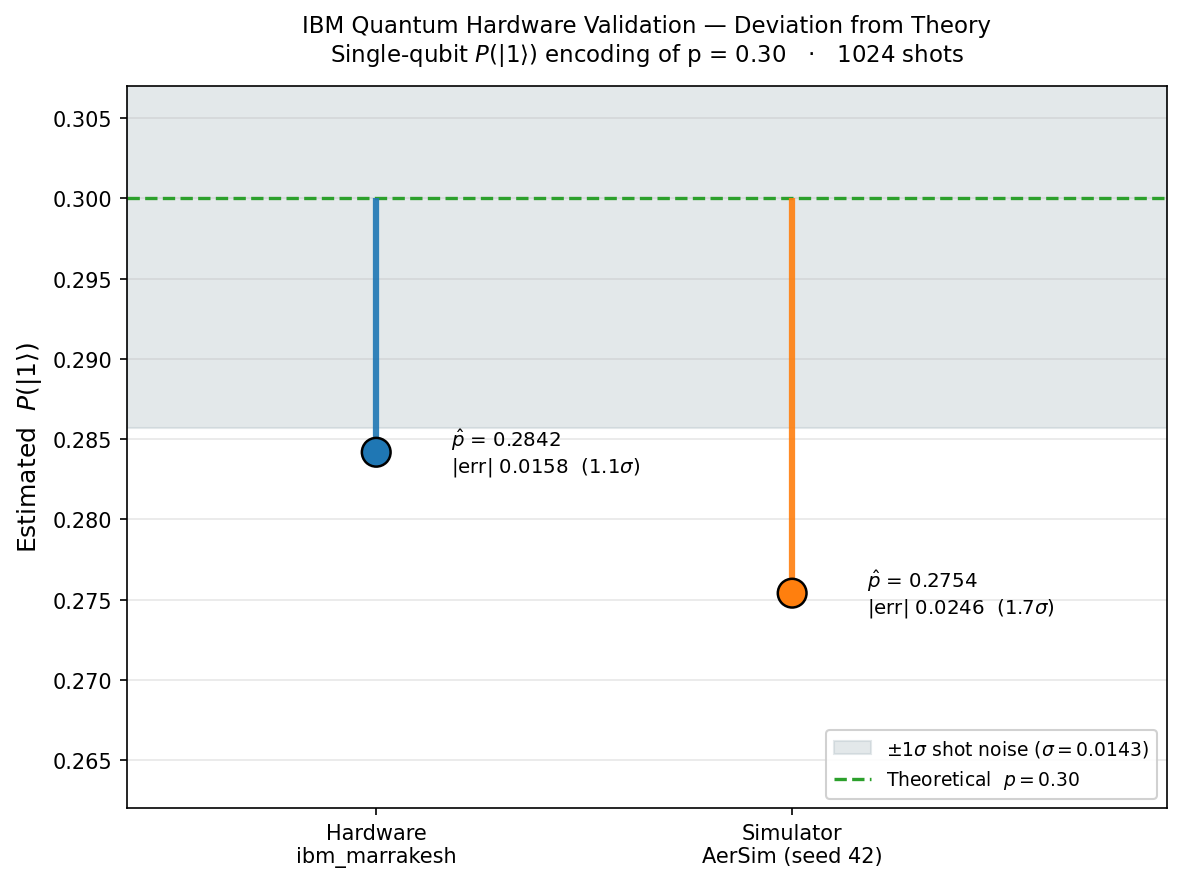
\includegraphics[width=0.8\textwidth]{figures/hardware_validation_plot.png}
\caption{Hardware validation as deviation from theory. Both the
\texttt{ibm\_marrakesh} hardware estimate ($|\text{err}| = 0.0158$, $1.1\sigma$)
and a matched simulator draw ($|\text{err}| = 0.0246$, $1.7\sigma$) fall within
the $\pm 1\sigma$ shot-noise band ($\sigma = 0.0143$) around the theoretical
$p = 0.30$. The hardware deviation is consistent with shot noise --- no
detectable device error at this scale. Job ID \texttt{d8nvd2bqv2lc7389d9e0},
1024 shots.}
\label{fig:hardware}
\end{figure}

% =====================================================================
\section{Discussion}
% =====================================================================
The results are best read as a separation of error sources. At NISQ scale the
total QAE pricing error decomposes into a discretization floor set by the number
of uncertainty qubits and a noise-dependent term that grows with the depolarizing
rate. Our sweep shows the floor alone is already $20\times$ above the precision
target, and the noise term overtakes even the floor by $p = 5\times10^{-3}$.
Increasing $n$ to lower the floor multiplies circuit depth and therefore the
accumulated noise, so the two error sources cannot be reduced independently on
near-term hardware.

This reframes the break-even question. The canonical analysis asks at what query
budget $M$ the $O(1/M)$ quantum estimator overtakes the $O(1/\sqrt{N})$ classical
one, holding the target precision $\varepsilon$ fixed and assuming $\varepsilon$
is the only error. Our data show that on hardware small enough to run,
$\varepsilon$ is not the only error and is not even the dominant one. A
budget-based crossover computed under the noiseless assumption therefore
describes a regime that current devices cannot enter.

The noise-invariance of the oracle-query depth sharpens this point. Because IQAE
does not lengthen its query schedule under noise, a practitioner monitoring only
the query budget would observe the algorithm terminating on schedule and
reporting a confident estimate, with no indication that the estimate has drifted
by dollars. Any honest break-even accounting must track delivered accuracy, not
query count, under realistic noise.

\paragraph{Limitations.}
The depolarizing model omits idling, crosstalk, and readout error, and the
hardware validation exercises only the single-qubit encoding step rather than the
full transpiled pipeline; a full-circuit hardware run is the natural next step but
is beyond the open-plan runtime budget used here. The instances studied are
deliberately small ($n = 3$), matching what near-term hardware can execute; the
discretization floor we identify would recede at larger $n$ on fault-tolerant
hardware, where this paper's near-term conclusions no longer apply.

% =====================================================================
\section{Conclusion}
% =====================================================================
We have measured, rather than assumed, the conditions under which QAE prices
European options accurately on near-term hardware. Under realistic depolarizing
noise the mean price error exceeds the $\varepsilon = 0.01$ precision target by
$66\times$ at current IBM error rates, and by $20\times$ even with no noise at
all, because the three-qubit discretization imposes an irreducible floor. The
oracle-query depth that the break-even analysis tracks is noise-invariant, so the
cost metric gives no warning as accuracy decays. A single-qubit run on
\texttt{ibm\_marrakesh} confirms the amplitude-encoding step is faithful to
within shot noise, locating the degradation in depth and discretization rather
than the encoding itself. The practical conclusion is that the QAE
option-pricing break-even, evaluated under near-term conditions, lies entirely
within the regime where QAE offers no usable advantage --- a finding that
motivates comparison against variance-reduced classical estimators, which we take
up in companion work.

% =====================================================================
\begin{thebibliography}{8}
% =====================================================================
\bibitem{stamatopoulos2020}
Stamatopoulos, N., Egger, D.J., Sun, Y., Zoufal, C., Iten, R., Shen, N., Woerner, S.:
Option pricing using quantum computers. Quantum \textbf{4}, 291 (2020)

\bibitem{woerner2019}
Woerner, S., Egger, D.J.: Quantum risk analysis. npj Quantum Information
\textbf{5}(1), 15 (2019)

\bibitem{grinko2021}
Grinko, D., Gacon, J., Zoufal, C., Woerner, S.: Iterative quantum amplitude
estimation. npj Quantum Information \textbf{7}(1), 52 (2021)

\bibitem{brassard2002}
Brassard, G., H{\o}yer, P., Mosca, M., Tapp, A.: Quantum amplitude amplification
and estimation. Contemporary Mathematics \textbf{305}, 53--74 (2002)

\bibitem{montanaro2015}
Montanaro, A.: Quantum speedup of Monte Carlo methods. Proceedings of the Royal
Society A \textbf{471}(2181), 20150301 (2015)

\bibitem{rebentrost2018}
Rebentrost, P., Gupt, B., Bromley, T.R.: Quantum computational finance: Monte
Carlo pricing of financial derivatives. Physical Review A \textbf{98}(2), 022321
(2018)

\bibitem{preskill2018}
Preskill, J.: Quantum computing in the NISQ era and beyond. Quantum \textbf{2},
79 (2018)

\bibitem{qiskit2024}
Qiskit contributors: Qiskit: An open-source framework for quantum computing
(2024)
\end{thebibliography}

\end{document}
